\chapter[\ee\ for \avr devices]{\ee\ for \avr\ devices}
\label{cha:singlecpu}

\section{The \rtd\ and \ee\ design flow}


The typical development environment provided by Atmel for the software
development for the \avr\ microcontrollers is composed by the Atmel
AVR Studio. Atmel AVR Studio is a development environment for
Microsoft Windows which integrates a source code editor, an
instruction set simulator and a debugger.

In addition to the traditional development flow, Evidence Srl provides
a design and configuration environment named \rtd, based on Eclipse
\cite{Eclipse}. Eclipse is an open framework initially developed by
IBM, which allows the possibility of integrating various development
tools in a common environment.

For that reason, when developing an application for \ee\, the
user is supposed to write the source code inside the \rtd\ IDE (see
Figure \ref{fig:eclipse_avr5_workspace}).

\begin{figure}
  \begin{center}
    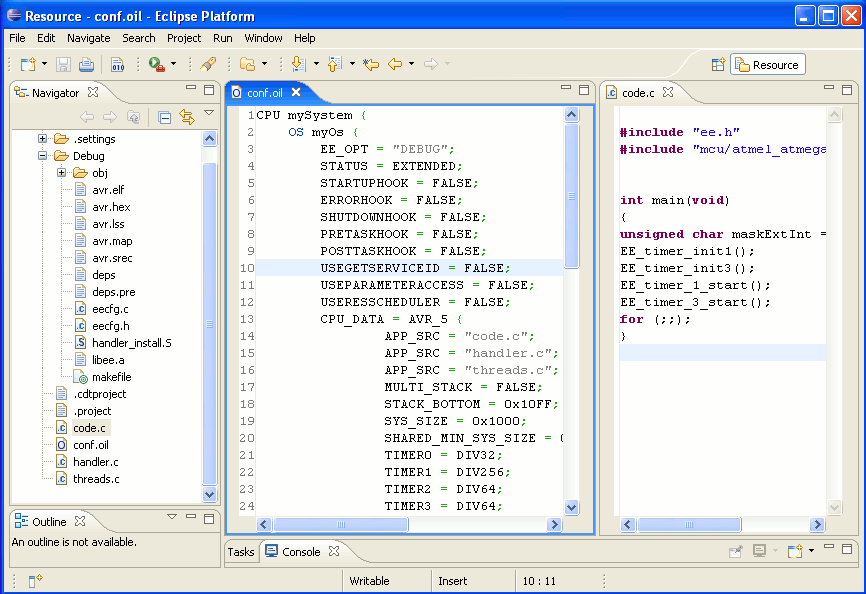
\includegraphics[width=12cm, bb=0 0 866 594]{images/eclipse_avr5_workspace.png}
  \end{center}
  \caption{The Eclipse workspace and the \rtd\ plugins for \avr.}
  \label{fig:eclipse_avr5_workspace}
\end{figure}

Application compilation is also done inside the Eclipse Framework. In
fact, the \rtd\ code generator is able to generate the \ee\
configuration files together with a set of configuration files
(typically, a \file{makefile} plus a set of \file{.c} files) which are
then used to compile the source code.

After that, compilation is started automatically by pressing on the
``Build Project'' menu item inside the ``Project'' menu, which
automatically calls the underlying \file{make} application provided by
the Cygwin environment. As an alternative, the ``Build Project''
command is also available by right clicking on the project name.

The choice of the Cygwin environment has been done to simplify the
building process of an application: in fact, Cygwin provides a set of
traditional Unix tools like \file{make}, \file{awk}, \file{sed}, which
are really useful to implement a command line application building
framework. Moreover, these tools are typically available for free on
the Linux platform, easing in this way the porting of the application
to a free development environment such as Linux.


\subsection{Building an application from command line}
The \rtd\ plugins provide three ways to develop an application:
\begin{enumerate}
\item A graphical interface to simplify the development of an
  application, based on Eclipse.
\item A scripting interface based on Apache ANT \cite{ANT}, which is
  the default scripting environment used in the Eclipse Framework.
\item A standalone code generator, that does not use Eclipse.
\end{enumerate}

Using ANT or the standalone version, the developer can automatically
generate from scripts the configuration data and the makefiles which
are then used to compile the application. This removes the need of
opening the graphical environment to compile an application, providing
a way to implement automatic compilation scripts and regression tests.

Please refer to the \rtd\ reference manual for information about ANT
scripting.



\section{Setting up the compiling environment for \avr}

\ee\ has been designed to be compiled using the GNU gcc toolchain.
The \avr\ porting of \ee\ in particular can be compiled using the GNU
tools for \avr. The porting provides both the \const{binutils} package
and the \const{gcc} package, plus a set of libraries which can be used
to control the various peripherals provided by the \avr\
microcontrollers.

The following list describes the various packages which contains the
various parts of the compilation toolchain:
\begin{description}
\item[The GNU assembler and binutils.] This package is distributed
  inside the AVRGCC package.
\item[The GNU AVR-GCC.] The GNU assembler, binutils and compiler are
  available as a part of the WinAVR suite {\em AVRGCC Compiler}, which
  is available as project on surceforge \url{http://winavr.sourceforge.net/}.

\item[C Libraries.] A set of libraries which can be used to control
  the peripherals implemented on the particular avr5 chip in
  use. These libraries are packaged together with the AVR-libc.
\end{description}

To compile an \ee\ application, the development
environment needs to be configured to correctly recognize the AVR-Gcc
compiler. For doing so, please go to the ``Preference'' menu, as shown
in Figure \ref{fig:preferences-menu}, and find the ``RT-Druid/Oil/Avr5
Configurator'' form as depicted in Figure \ref{fig:preferences-avr5}.
The first textbox, labeled \const{Gcc path}, refers to the
installation directory of the AVR-Gcc compiler.  The second and third
textboxes are useful if you are using a development environment based
on the Crossbow Mib5x0 board. In particular, the second textbox,
labeled \const{Uisp path}, refers to the installation directory of the
uisp programmer for Crossbow Mib5x0 board, and the third textbox,
labeled \const{Serial port device}, refers to the COM serial port
where the board is attached.


\begin{warning}
The install directories specified in the two textboxes of Figure
\ref{fig:preferences-avr5} does {\em not} include the \file{bin}
directory! 

That is, \file{c:\\WinAVR-20071221} is correct, wheras
\file{c:\\Programmi\\WinAVR-20071221\\bin} is not.
\end{warning}


\begin{figure}[htb]
\begin{center}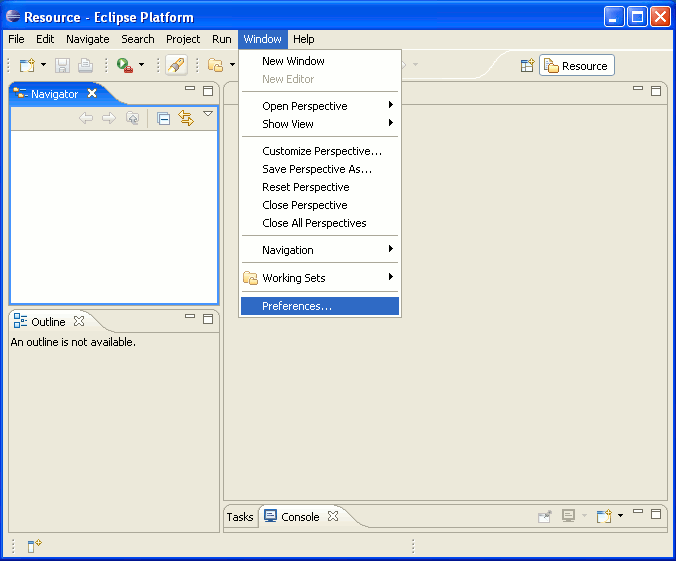
\includegraphics[
  width=8cm, bb=0 0 676 561]{images/preferences_menu.png}\end{center}
\caption{Go to the ``Preference'' menu.}
\label{fig:preferences-menu}
\end{figure}

\begin{figure}[htb]
\begin{center}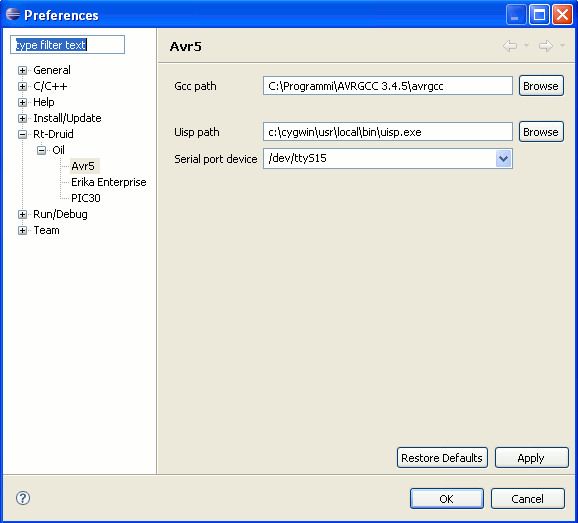
\includegraphics[
  width=8cm, bb=0 0 578 523]{images/preferences_avr5.png}\end{center}
\caption{Select paths for compiler and assembler.}
\label{fig:preferences-avr5}
\end{figure}


\section{Writing software for \avr\ using \ee}

\begin{note}
Writing an application for \avr\ using \ee\ is
very simple. Please refer to the \ee Tutorial for the \avr\
architecture for a step-by-step guide with screenshots on how to
create, compile and debug a \avr\ application written with \ee.
\end{note}

This section describes the details about the various
configuration options which are available to create and compile an
\ee\ application for a \avr\ microcontroller.

\begin{note}
For a complete description of all the OIL parameters, please refer to
the \rtd\ reference manual.
\end{note}

\subsection{Avoid the generation of dependency files}
The typical compilation process of an \ee\ application involves the
computation of a dependency file which is used to understand which are
the files which needs to be compiled or updated.

To avoid the computation of these dependencies (useful when you are
sure you basically have to compile everything), you can put the
following line in the OIL file:

\begin{lstlisting}
CPU mySystem {
  OS myOs {
    EE_OPT = "NODEPS";
    ...
  };
  ...
};
\end{lstlisting}

\subsection{Avoid the generation of .src files from C files}
The typical compilation process of an \ee\ application produces
various files which can be used to better analyze the code generated
by the Avr-Gcc compiler. In particular, from each .C file, a .SRC file is
produced containing the corresponding assembler listing, which is then
compiled by the Avr-Gcc compiler to produce the .o.

It is possible to avoid the intermediate step which leads to the
production of the .SRC file. In that case, the compiler will be
responsible of producing the .O file directly from the .C file. This
in general also speeds up the compilation process a little bit.

To obtain that feature, you can put the following lines in the OIL
file.

\begin{lstlisting}
CPU mySystem {
  OS myOs {
    EE_OPT = "NOSRC";
    ...
  };
  ...
};
\end{lstlisting}

\subsection{Printing the commands executed (verbose mode)}

The default compilation process typically prints only a compact output
for each compilation step. That is in general not useful whenever a
file is not compiled properly and the user wants to know the exact
command which is executed in the compilation process.

To obtain a printing of the complete list of commands issued by the
\ee\ makefile, you can add the following line to the OIL file:

\begin{lstlisting}
CPU mySystem {
  OS myOs {
    EE_OPT = "VERBOSE";
    ...
  };
  ...
};
\end{lstlisting}

\subsection{Source files composing an application}
The source files which can be put in an \rtd\ project are composed by
C-language files (with extension \file{.c}) and Assembler files (with
extension \file{.S}). Assembler files are always preprocessed by the C
preprocessor. All the application files which has to be included in
the final application needs to be listed inside the OIL file, as in
the following OIL example:

\begin{lstlisting}
  ...
  CPU_DATA = AVR5 {
    ...
    APP_SRC = "file_1.c";
    APP_SRC = "file_2.c";
  };
  ...
\end{lstlisting}

% /toOl: commented
%\nb{inserire screenshot del configuratore grafico!!}



\subsection{Stack handling}
\ee\ can be configured as monostack or multistack.

In a monostack configuration, only a single stack exists in the
system. No blocking primitives are supported, and all the tasks and
interrupts execute on the same stack. In this case, the one and only
stack starts from the top of the application allocated memory, growing
towards higher addresses. The monostack configuration can {\em not} be
used if the application needs to call RTOS primitives such as
\fn{WaitSem} and \fn{WaitEvent}. Moreover, it cannot be used when \ee\
conformance classes ECC1 and ECC2 are used.

To configure a monostack kernel in the OIL file, the user has to write
the following lines:

\begin{lstlisting}
  ...
  CPU_DATA = AVR5 {
    ...
    MULTI_STACK = FALSE;
  };
  ...
\end{lstlisting}


In a multistack configuration, the kernel support the existence of
different stacks in the same application. Having different stacks
allow the application tasks to use blocking primitives like
\fn{WaitSem} and \fn{WaitEvent}, which basically may block the
execution of the running task. In that case, the calling task must have
a {\em private} stack which is changed upon blocking. The stack will
be selected again when the task will be rescheduled. There are
different stacks available in a multistack configuration:
\begin{itemize}
\item A shared stack (used by all the tasks which have a shared
  stack);
\item An IRQ stack (used by all the ISR Type 2 routines);
\item A set of private stacks (one for each task which has selected a
  private stack).
\end{itemize}

In the \avr\ architecture, the shared stack works as in the monostack
configuration, that is it is allocated at the end of the SRAM data memory, 
growing towards lower addresses. The IRQ stack and the private stacks, instead,
are allocated in the application data space as arrays.
The following example shows an OIL configuration which configures a
multistack kernel without a separate IRQ stack (in this case, IRQ
handlers execute on the stack of the interrupted task):

\begin{lstlisting}
  ...
  CPU_DATA = AVR5 {
    ...
    MULTI_STACK = TRUE {
      IRQ_STACK = FALSE;
    };
  };
  ...
\end{lstlisting}
The following example shows an OIL configuration which configures a
multistack kernel with a separate IRQ stack (in this case, some
registers are saved on the stack of the interrupted task, but the IRQ
handler C function is executed on a separate IRQ stack).
In this example is showed also the task0 that uses a private stack.

\begin{lstlisting}
  ...
  CPU_DATA = AVR5 {
    ...
    MULTI_STACK = TRUE {
      IRQ_STACK = TRUE {
	SYS_SIZE=64;
      };
    };
  };
  ...
  TASK Task0 {
  ...
   STACK = PRIVATE {
   	SYS_SIZE=64;
   };
  ...		   
  };
  ...
\end{lstlisting}

% /toOl: commented
%\nb{inserire screenshot del configuratore grafico!!}

\subsection{Interrupt handling}
\ee\ for \avr\ provide support for fast Interrupt Service
Routines (ISR) which do not require any RTOS primitive to be called,
as well as regular ISRs, which can call RTOS primitives (e.g., a timer
interrupt can call \fn{ActivateTask} to activate a periodic task). The
first kind of ISRs are called {\em ISR Type 1}, and always have
hardware interrupt priority greater than the second kind of ISRs which
are called {\em ISR Type 2}.

To declare an ISR of tipe 1 or 2, the user have to specify inside the
OIL file a set of parameters: the interrupt source used by the
interrupt, the type of ISR, and finally the handler function
associated with the interrupt.  For example if we want to declare a
ISR type 2 associated to the timer1 overflow interrupt we have to type
the following code inside the OIL file:

\begin{lstlisting}
  ...
  CPU_DATA = AVR5 {
    ...
    APP_SRC = "handler.c";
    ...
    MULTI_STACK = FALSE;
    HANDLER = HANDLER_T1_OVERFLW {	
      FUNCTION = "myfunction";
      TYPE = 2;
    };
  };
  ...
\end{lstlisting}

In the previous example the function \fn{myfunction__isr2} is a simple
C function, that is called everytime the timer1 overflow interrupt are
raised.  The strings that have to be used in the ATmega128 model of
AVR5 family are:

\begin{lstlisting}
   / * Interrupt Handlers  strings * /
    STRING HANDLER_IRQ0;	// external interrupt request 0
    STRING HANDLER_IRQ1;	// external interrupt request 1
    STRING HANDLER_IRQ2;	// external interrupt request 2
    STRING HANDLER_IRQ3;	// external interrupt request 3
    STRING HANDLER_IRQ4;	// external interrupt request 4
    STRING HANDLER_IRQ5;	// external interrupt request 5
    STRING HANDLER_IRQ6;	// external interrupt request 6
    STRING HANDLER_IRQ7;	// external interrupt request 7
    STRING HANDLER_T0_MATCH;	// Timer/Counter 0 Compare Match
    STRING HANDLER_T0_OVERFLW;	// Timer/Counter 0 Overflow
    STRING HANDLER_T1_EVENT;	// Timer/Counter 1 Capture Event
    STRING HANDLER_T1_MATCH_A;	// Timer/Counter 1 Compare Match A
    STRING HANDLER_T1_MATCH_B;	// Timer/Counter 1 Compare Match B
    STRING HANDLER_T1_MATCH_C;	// Timer/Counter 1 Compare Match C
    STRING HANDLER_T1_OVERFLW;	// Timer/Counter 1 Overflow
    STRING HANDLER_T2_MATCH;	// Timer/Counter 2 Compare Match
    STRING HANDLER_T2_OVERFLW;	// Timer/Counter 2 Overflow
    STRING HANDLER_T3_EVENT;	// Timer/Counter 3 Capture Event
    STRING HANDLER_T3_MATCH_A;	// Timer/Counter 3 Compare Match A
    STRING HANDLER_T3_MATCH_B;	// Timer/Counter 3 Compare Match B
    STRING HANDLER_T3_MATCH_C;	// Timer/Counter 3 Compare Match C
    STRING HANDLER_T3_OVERFLW;	// Timer/Counter 3 Overflow
    STRING HANDLER_SPI; 	// SPI Serial Transfer Complete
    STRING HANDLER_US0_RX;  	// USART0 Rx complete
    STRING HANDLER_US0_EMPTY;	// USART0 Data Register Empty
    STRING HANDLER_US0_TX;  	// Usart0 Tx complete
    STRING HANDLER_US1_RX;  	// USART1 Rx complete
    STRING HANDLER_US1_EMPTY;	// USART1 Data Register Empty
    STRING HANDLER_US1_TX;  	// Usart1 Tx complete
    STRING HANDLER_ADC; 	// ADC Conversion Complete
    STRING HANDLER_EEPROM;	// EEPROM Ready
    STRING HANDLER_ANALOG_COMP;	// Analog Comparator
    STRING HANDLER_2WSI;	// Two-wire serial Interface
    STRING HANDLER_SPM_READY;	// Store program Memory Ready
\end{lstlisting}

Please remember that the \avr\ family of microcontroller has an
interrupt vector table which is stored in the flash memory. The lowest
addresses of the interrupt vector table is allocated to the Reset and
to the interrupt vectors. Interrupt handlers placed at lower addresses
has higher hardware priorities than interrupt handlers placed at
higher addresses.

Writing an ISR 2 or ISR 1 with \ee\ implies that :
\begin{itemize}
\item An assembler stub will be generated for the ISR. The ISR stub
  will have the name of the ISR (in the example,
  \fn{__isr2_myfunction}). The assembler stub will call a C function
  named \fn{myfunction}, which is provided by the user inside the
  application C files. The assembler stub will be attached to the
  interrupt of the peripheral (in the example, timer 1). Every time an
  interrupt for the peripheral arrives, the assembler stub will
  execute, which in turns calls the internal C function whose body has
  been specified by the user.
\item The assembler stub saves {\em all} the CPU registers on the
  current stack. After that, if a multistack configuration with
  private IRQ stack has been selected, the stack is changed to a
  private IRQ stack. Otherwise, the ISR will execute on the stack of
  the running task, as in the ISR1 case.  At the end of the stub, the
  \ee\ end IRQ function will be executed to choose which is the next
  task to run.
\end{itemize}

To use the external interrupt source the user must setting the external 
interrupt mask with the following function. 

\begin{function_nopb2}{EE\_IC\_enable\_external\_IRQ}{EE_IC_enable_external_IRQ:avr5}
  \synopsis{void EE_IC_enable_external_IRQ(EE_TYPEIRQMASK i);}
  \begin{fundescription}
    Enables the external interrupt source that are specified in the
    8-bit bitmask. For example, if the third bit in the bitmask is
    set, the third external interrupt will be enabled.
  \end{fundescription}
\end{function_nopb2}


\begin{function_nopb2}{EE\_IC\_clear\_pending\_IRQ}{EE_IC_clear_pending_IRQ:avr5}
  \synopsis{void EE_IC_clear_pending_IRQ(void);}
  \begin{fundescription}
    Clears ALL the pending interrupts.
  \end{fundescription}
\end{function_nopb2}

\subsection{\avr timers}

The number of hardware timers in the \avr family is highly dependent
on the particular chip used. For example, the ATmega128 device has 4
timers (2 8-bit timers and 2 16-bit timers).

The timers used in the application with the corresponding prescalers
can be specified in the OIL file (these settings applies to \avr\
atmega128.

The following example show how to configure a set of timers for an
\avr\ atmega128.

\begin{lstlisting}
  ...
  CPU_DATA = AVR5 {
    ...
    TIMER0 = DIV32;
    TIMER1 = DIV8;
    TIMER2 = DIV64;
    TIMER3 = DIV1;
    ...
  };
  ...
\end{lstlisting}
	
The prescaler factor for timers in ATmega128 model are \const{DIV1},
\const{DIV8}, \const{DIV64}, \const{DIV256}, and \const{DIV1024}.  The
timer0 have also the prescaler factor \const{DIV32}.
The User can use inside the source code of application the following 
functions to use the timer.

\begin{function_nopb2}{EE\_timer\_initx}{EE_timer_initx:avr5}
  \synopsis{void EE_timer_initx(void);}
  \begin{fundescription}
    Inizialize the timerx (x = 0,1,2,3)
  \end{fundescription}
\end{function_nopb2}
  
\begin{function_nopb2}{EE\_timer\_x\_start}{EE_timer_x_start:avr5}
\synopsis{void EE_timer_x_start(void);}
\begin{fundescription}
  Start the timerx (x = 0,1,2,3)
\end{fundescription}
\end{function_nopb2}

\begin{function_nopb2}{EE\_timer\_x\_stop}{EE_timer_x_stop:avr5}
\synopsis{void EE_timer_x_stop(void);}
\begin{fundescription}
    Stop the timerx (x = 0,1,2,3)
\end{fundescription}
\end{function_nopb2}

\begin{function_nopb2}{EE\_timer\_x\_get}{EE_timer_x_get:avr5}
\synopsis{EE_UREG EE_timer_x_get(void);}
\begin{fundescription}
    Return the value of the counter register of the timerx (x = 0,1,2,3)
\end{fundescription}
\end{function_nopb2}
  
\subsection{Configuring a particular \avr\ microcontroller}

Atmel produces various versions of the \avr\ microcontrollers, each
one with different peripherals and memory sizes.

The AVR-Gcc specifies the various peripherals and memory areas by
passing an appropriate command line parameter which selects the right
linker script for the specified device. For that reason, the OIL file allows 
the specification of the microcontroller used, as in the following example:

\begin{lstlisting}
  ...
  MCU_DATA = AVR5 {
    MODEL = ATMEGA128;
  };
  ...
\end{lstlisting}

Currently, \ee\ supports the following values for the \const{MODEL}
attribute:
\begin{itemize}
\item AVR5 devices: \newline
  \const{ATMEGA128},\newline
\end{itemize}



\section{Configuring the EDF scheduler}

When configuring the EDF kernel for an \ee\ application, the user has
the possibility to specify the tick length in the OIL file to allow
the specification of a relative deadline using a temporal value.

In particular, the user can specify a tick value as follows:

\begin{lstlisting}
 KERNEL_TYPE = EDF {TICK_TIME = "125ns";};
\end{lstlisting}

and then specify a relative deadline using a timing value as follows:

\begin{lstlisting}
 TASK myTask1 {
   REL_DEADLINE = "10ms";
 };
\end{lstlisting}

The \rtd\ code generator will handle the the conversion between the
relative deadline value in the corresponding timing value
automatically.

The important thing in this process is to correctly specify the
\const{TICK_TIME}. In general, that value depends on the timing
reference which is made available by the \avr. The current timing
reference implemented in the EDF kernel for \avr\ is based on the
value of the 16 bit timer Timer1.

The 16 bit timer is obtained by using the timer1 available on the
\avr.  The clock used for the timers is the system clock, with a tick
time equal to $\frac{1}{F_{c}}$. $F_c$ is the frequency of the
oscillator, and depends on the application configuration.

In the case of the Atmel ATmega128, the default frequency is 8 MHz. In
that case, the OIL file should contain the following line:
\begin{lstlisting}
 KERNEL_TYPE = EDF {TICK_TIME = "125ns";};
\end{lstlisting}
and the \fn{main()} function should have the following line before
using any \ee\ primitive:
\begin{lstlisting}
  EE_timer1_init();
  EE_timer1_start();
\end{lstlisting}



